\documentclass{standalone}
\usepackage{hsbcommon}
\makeatletter\AtBeginDocument{\@buildstepset{1,2,3,4,5,6}}\makeatother
\usepackage{tikz}
\usetikzlibrary{fit}
\begin{document}
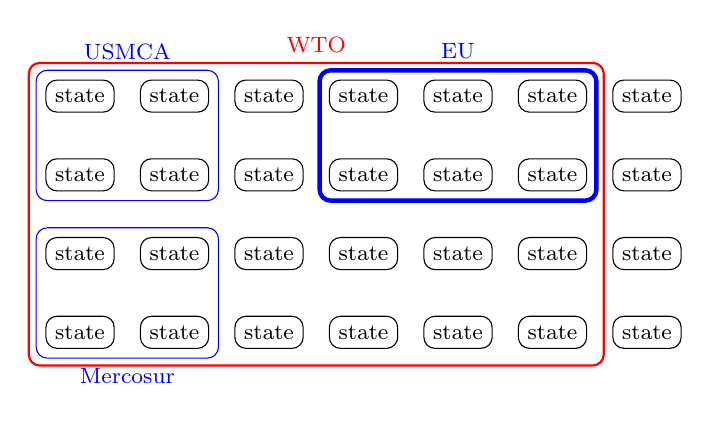
\begin{tikzpicture}
    \tikzset{
        every node/.style={
            draw,
            rounded corners,
            font=\footnotesize
        }
    }
    \foreach \x in {1,2,3,4,5,6,7}
    \foreach \y in {1,2,3,4}
    {
        \node (X\x-Y\y) at (1.2*\x,\y) {state};
    }
    \ifstep{1}{
        \begin{scope}[red]
            \node [thick,fit={(X1-Y4) (X6-Y1)},label=above:WTO,inner sep=6pt] {};
        \end{scope}
    }
    \ifstep{2}{
        \begin{scope}[blue]
            \node [fit={(X1-Y4) (X2-Y3)},label=above:USMCA] {};
            \node [fit={(X1-Y2) (X2-Y1)},label=below:Mercosur] {};
            \node [fit={(X4-Y4) (X6-Y3)},label=above:EU,ultra thick] {};
        \end{scope}
    }

    
\end{tikzpicture}
\end{document}